\documentclass[12pt,a4paper]{article}

\usepackage[utf8]{inputenc}
\usepackage{amsmath, amssymb, amsthm}
\usepackage{graphicx}
\usepackage{float}
\usepackage{booktabs}
\usepackage{siunitx}
\usepackage{hyperref}
\usepackage{natbib} % or biblatex if you prefer
\bibliographystyle{apa} % set APA style

\title{Benchmarking Time Series Clustering Using Simulated Data}
\author{Rasika Dilhani}
\date{\today}


\begin{document}
	\maketitle
	
	\section*{Meeting Tasks to Study}
	
	\begin{itemize}
		\item Propose the parametric space of the simulation study.  
		Based on previous experience, very long time series can be problematic; a sample size of around 1000 data points may be more suitable for analysis.
		
		\item Review details about the ECG datasets already found and answer the question:  
		\textit{Are these data already clustered/classified in the literature?}
		
		\item Always bring validated, high-quality references and citations.
		
		\item Identify another possible dataset for clustering/classification.
		
		\item Browse carefully through \url{http://www.timeseriesclassification.com}.
		
		\item Create a benchmark for time series clustering using simulated data:
		\begin{itemize}
			\item Explore different ARMA models (varying series lengths and parameters).
			\item Investigate the "addition" of deterministic chaos.
		\end{itemize}
		
	\end{itemize}

	
\section{Parametric space}
  
Based on previous experience, very long time series can be problematic; a sample size of around 1000 data points may be more suitable for analysis.

\section{Details of ECG datasets}
Each record includes the ECG signals measured from both the left and right sides of the thorax. Consequently, every entry in this dataset is represented as a two-dimensional time series that characterizes a type of non-invasive fetal ECG.  More details of \url{https://www.physionet.org/content/challenge-2013/1.0.0/}

\section{Publicly available another datasets}
The GitHub page at \url{https://github.com/awesomedata/awesome-public-datasets/tree/master} contains a variety of datasets that can be used for time series analysis. This GitHub repository offers a comprehensive, topic-centric listing of public, high-quality datasets collected from numerous sources. The datasets cover a wide range of domains including agriculture, climate, economics, healthcare, biology, machine learning, finance, transportation, and more, making it easy to find relevant data for particular analytical tasks.

\subsection{Time Series Datasets}
Dedicated sections, such as "TimeSeries" and "Economics," feature datasets suitable for time series analysis, including:

\textbf{Time Series Data Library (TSDL):} Contains diverse time series data for statistical modeling and forecasting.

\textbf{UC Riverside Time Series Dataset:} Offers benchmark datasets for classification, clustering, and time series prediction.

\textbf{Hard Drive Failure Rates:} Useful for reliability analysis over time.


Additional datasets in climate, energy, finance, and transportation (like airline and bike share data) are also frequently time-indexed, and can be leveraged for time series or longitudinal studies. 

\section{Introduction to simulated time series data}
Time series clustering plays a crucial role in understanding complex dynamic systems, both in research and in everyday applications such as healthcare, finance, energy management, and climate monitoring. Based on the previous research experience in this regards on our proposal, while we work primarily with real-world datasets, it is essential to first establish a benchmark framework using simulated data. Simulated datasets allow controlled variation of parameters such as noise, series length, and complexity, enabling systematic evaluation of clustering algorithms and ensuring reproducibility. By uncovering hidden structures, detecting patterns, and grouping similar temporal behaviors, time series clustering facilitates exploratory analysis, anomaly detection, and improved decision-making in systems where labeling is costly or unavailable. Establishing a validated benchmark provides a foundation for applying clustering methods confidently to real data, enhancing the reliability and interpretability of experimental results.
	
\section{Methodology}
In this study, ordinal patterns were utilized for time series clustering. The experiments were conducted using simulated ARMA processes with a range of sample sizes (500, 1000, 1500, 2000, and 5000). For the initial analysis, the ARMA model parameters were fixed at AR = 0.6 and MA = 0.3, while the embedding dimension (D) was systematically varied from 3 to 6 to investigate its influence on the ordinal pattern-based measures.

Based on the results obtained from these experiments, an embedding dimension of 5 (D = 5) with a fixed sample size of 1000 was determined to be representative for deeper investigation. Subsequently, a second set of experiments was conducted in which the ARMA model parameters were varied, enabling assessment of the effect of different AR and MA configurations on the clustering characteristics derived from ordinal pattern analysis.

This approach allowed for a comprehensive evaluation of how both sample size and embedding dimension impact the application of ordinal patterns in time series clustering, as well as how sensitive the results are to underlying ARMA model dynamics. 


\section{Results and Discussion}
The results from these experiments are summarized as follows. The first five figures illustrate the outcomes when the ARMA model parameters are fixed (AR = 0.6, MA = 0.3), highlighting the effects of different sample sizes (500, 1000, 1500, 2000, and 5000) and embedding dimensions (ranging from 3 to 6) on the clustering performance using ordinal patterns.

Subsequently, based on these preliminary results, embedding dimension 5 and a sample size of 1000 were selected for a more detailed study of how clustering characteristics change when the ARMA model parameters are varied. The following figures present these findings, demonstrating the sensitivity of ordinal pattern-based clustering to underlying time series dynamics as governed by the AR and MA coefficients.

These visualizations collectively showcase how sample size, embedding dimension, and model parameters interact to influence the entropy and complexity measures derived from ordinal pattern analysis, providing insights for optimal parameter selection in practical time series clustering applications.

\begin{figure}[H]
	\includegraphics[width=0.8 \textwidth]{d3 different sample size}
	\caption{$H \times C$ Plane with Embedding dimension 3}
	\label{fig:HC Plane D3}
\end{figure}	

\begin{figure}[H]
	\includegraphics[width=0.8 \textwidth]{d4 different sample size}
	\caption{$H \times C$ Plane with Embedding dimension 4}
	\label{fig:HC Plane D4}
\end{figure}

\begin{figure}[H]
	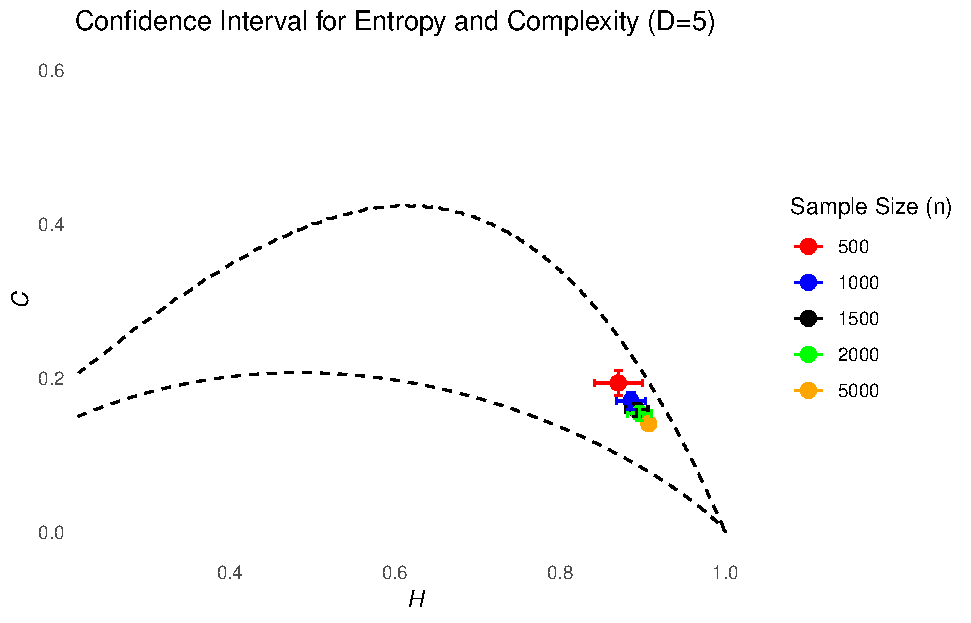
\includegraphics[width=0.8 \textwidth]{d5 different sample size}
	\caption{$H \times C$ Plane with Embedding dimension 5}
	\label{fig:HC Plane D5}
\end{figure}

\begin{figure}[H]
	\includegraphics[width=0.8 \textwidth]{d6 different sample size}
	\caption{$H \times C$ Plane with Embedding dimension 6}
	\label{fig:HC Plane D6}
\end{figure}			
	
\begin{figure}[H]
	\includegraphics[width=0.8 \textwidth]{different ARMA parameters}
	\caption{ARMA parameter changes}
	\label{fig:HC Plane for different parameters}
\end{figure}	
	
\section{Conclusion and future work}
These experiments show that using ordinal patterns can help group (cluster) time series data in meaningful ways. First, we kept the model settings the same (AR = 0.6 and MA = 0.3) and changed the sample size (from 500 up to 5000) and the embedding dimension (from 3 to 6) to see how these factors affect measures like entropy and complexity. Then, we focused on one case (embedding dimension 5 and sample size 1000) and changed the ARMA model’s parameters. The results suggest that the way we group time series using ordinal patterns depends on the sample size, the embedding dimension, and the ARMA model’s settings.

Future Work
In the future, I plan to include experiments with deterministic chaos (using time series with chaotic behavior) as well as random data. This will help test whether ordinal patterns and complexity-entropy measures can tell the difference between chaos and randomness, and improve clustering results in these new situations.
	
%	\bibliography{yourbibfile}
	
\end{document}

